\documentclass{ceurart}
\sloppy
\usepackage{listings}
\lstset{breaklines=true, keywordstyle=\bfseries}
\usepackage[inline]{enumitem}
\usepackage{tikz}
\usepackage{setspace}

\begin{document}

\copyrightyear{2024}
\copyrightclause{Copyright for this paper by its authors. Use permitted under Creative Commons License Attribution 4.0 International (CC BY 4.0).}
\conference{ITADATA 2024 - BigHPC, Pisa, Italy - 17-19 September 2024}
\title{Quantum-Classical Sentiment Analysis}
\author[1]{Mario Bifulco}[email=mario.bifulco@edu.unito.it,url=https://github.com/TheFlonet]
\author[1]{Luca Roversi}[orcid=0000-0002-1871-6109,email=luca.roversi@unito.it,url=https://www.di.unito.it/~rover/]
\address[1]{Università degli studi di Torino, Dipartimento di Informatica, Corso Svizzera 185 - 10149 Torino}

\begin{abstract}
    The following work explores the advantages of a hybrid classical-quantum solver, particularly applied to sentiment analysis. Additionally, we have developed an alternative hybrid solver to leverage the quantum component of the computational infrastructure further. 
    The experimental results collected show how quantum computation allows faster convergence to optimal solutions and how effective hybrid solvers can be developed to avoid the opaque systems proposed by D-Wave, thus making greater use of the quantum component.
\end{abstract}
\begin{keywords}
    Quantum Adiabatic Computing \sep 
    Machine Learning \sep
    Sentiment Analysis \sep 
    Hybrid solver 
\end{keywords}

\maketitle

\begin{spacing}{1}
\section{Introduction}
    In natural language processing, the two main challenges in developing new models are the difficulty in acquiring high-quality data and the extensive training times required to make models more expressive\cite{scaling}.

This work focuses on the latter issue. We experiment with unconventional computing architectures, the goal being to assess if and how they can help accelerate training time to obtain more expressive models. To this purpose, our choice is architectures that develop Adiabatic Quantum Computing (AQC). The reason is twofold, on one side AQC by its very nature solves minimization problems in the QUBO form (Quadratic Unconstrained Binary Optimization), on the other the core of many AI is minimizing some function by looking for the values of specific parameters.

We choose SVM\cite{SVM} over more standard Transformers models because preliminary investigations on using SVM for machine learning took leveraging AQC exists\cite{QSVM} and SVM share some similarities with the attention mechanism of Transformers\cite{TransformerSVM}.

Precalling that, among classification tasks in natural language processing, the binary version of Sentiment Analysis (BSA) aims to separate sentences that convey ``positive'' emotions from those that convey ``negative'' emotions. We reduced the BSA to QUBO and evaluated
\begin{enumerate*}
    \item performance during classification,
    \item the time required to train the model, and
    \item the time required to classify new examples,
\end{enumerate*}
compared to more standard techniques implemented with heuristics and classical architectures. To improve our results relative to training time we also started to investigate software-based alternatives to the proprietary mechanisms that physically embed QUBO problems on Quantum CPU (QPU) for AQC. We shall briefly report on this in the conclusion.

\section{Quantum Support Vector Machine for Sentiment Analysis}

We choose TweetEval\cite{TweetEval} to verify the effectiveness of SVM as QUBO for BSA. This dataset is considered a standard for comparing different models and contains a sufficiently large and representative number of labelled examples. The ``sentiment'' split of TweetEval includes three classes: positive, negative and neutral. We choose to discard all ``neutral'' samples to avoid introducing errors during learning due to examples belonging to non-expressive classes. Additionally, the quantity of elements in the positive and negative classes was normalized to ensure a balanced dataset.

Since SVMs do not natively support text processing, it is necessary to compute embeddings. Among the various possibilities, SentenceBert\cite{SentenceBert} allows for capturing the contextual information of the entire sentence by producing a single embedding.

For comparison with the classical counterpart, we choose 
\begin{enumerate*}
    \item the solver CPLEX\cite{cplex}, without modifying its parameters,
    \item RoBERTa\cite{ROBERTA}, a deep-learning model based on BERT\cite{BERT} and the attention mechanism\cite{Attention}.
\end{enumerate*}
RoBERTa allows for a fair comparison as it is pre-trained on TweetEval.

\begin{table}
    \caption{Classification results}
    \label{tab:classification}
    \begin{tabular}{cccc}
        \toprule
        & CPLEX & D-Wave & RoBERTa \\
        \midrule
        F1-Score (\%) & 76.9 & 76.1 & 94.3 \\
        Train time (s) & 101.9 & 39.2 & / \\
        Eval time (s) & 2.2 & 33.9 & 136.8 \\
        \bottomrule
    \end{tabular}
\end{table}

Table \ref{tab:classification} shows some data related to the training and inference of the different models compared. D-Wave stands for what we develop and report on here.

\paragraph{F1 score} The classification conducted by RoBERTa is significantly better, although the results of both CPLEX and D-Wave are also well above random guesses. The slight difference between the solution obtained with CPLER and that with D-Wave may be due to some limitations of the current hybrid solvers, which restricted the domain of the optimisation variables from real numbers to integers.

\paragraph{Training time} The time required by D-Wave to find an optimal assignment is 60\% less than that of the classical counterpart. Although not available, it is reasonable to expect an even better result if compared to the time required RoBERTa, which may require several hours of training on high-performance machines.

\paragraph{Prediction time} The complexity of the RoBERTa architecture also affects the time required for prediction by requiring more computing time than CPLEX or D-Wave. The higher time required is due to D-Wave returning a set of optimal solutions, for each of them a model is created to apply a majority vote to establish the class in inference. Experimentally, no advantages emerge from using such a procedure, known as ensemble learning, whereby it is possible to work with only the first of the optimal assignments produced, obtaining times comparable to those of CPLEX.

\section{Maximizing quantum boost}

Using the default hybrid solver entails an opaque workflow due to the underlying proprietary technology. Examination of the available data, however, shows that the QPU contributes very marginally in calculating the solution, averaging 0.08\%. Since the performance boost derives from the quantum component, it is worth considering whether it is possible to use a greater amount of it, ideally shifting the entire problem resolution onto the QPU and delegating only pre- and post-processing operations to the CPU.

Direct access to the QPU is possible provided you manually perform certain pre-processing operations of the problem such as:
\begin{enumerate}
   \item Convert the problem into QUBO form i.e,
    \begin{enumerate*}
        \item incorporates the constraints into the objective as penalty functions via appropriately parameterised Lagrangian relaxation\cite{QbridgeI},
        \item converts the optimisation variables into binary variables,
        \item transforms the objective function into a minimisation problem.
    \end{enumerate*}
    \item Search for the minor\cite{ME}\cite{MEdwave} associated with the QUBO problem that can be mapped onto the graph corresponding to the QPU Pegasus\cite{Pegasus}.
\end{enumerate}

By performing these steps independently, it is possible to bypass D-Wave's proprietary technology and maximise the use of the QPU. The only operation with high computational cost among those described is the search for the minor embedding, which is NP-complete. For this reason, the table \ref{tab:embedding} focuses on the time required to compute the minor embedding of the graph representing an SVM. We can see that, for 128 variables, the calculation takes more than 7 minutes and occupies about 40\% of the available qubits on the QPU, this makes the direct use of the QPU not applicable to real-size problems.

\begin{table}
    \caption{Embedding search time}
    \label{tab:embedding}
    \begin{tabular}{ccccccc}
        \toprule
        Problem nodes & 4 & 8 & 16 & 32 & 64 & 128 \\
        \midrule
        Embedding Nodes & 4 & 13 & 40 & 138 & 526 & 2117 \\
        Avg Time (s) & 0.2 & 0.3 & 0.6 & 6.1 & 53.4 & 434.2 \\
        \bottomrule
    \end{tabular}
\end{table}

\section{Homebrewing a Hybrid Solver}

Given the practical impossibility of using the QPU directly, it is unavoidable to rely on hybrid solvers. Therefore, we investigate a first attempt to design a hybrid solver, to maximize the use of the QPU.

Provided the structure of the QUBO problem, algebraic techniques can be employed to decompose the problem into smaller chunks. Once a sufficiently small problem is reached, it can be solved on the QPU, and the solutions of the sub-problems can then be aggregated.

This technique is not limited to SVM but applies more generally to a strategy for solving QUBO problems. Consequently, the subsequent considerations will examine matrices that do not necessarily represent an SVM.

\begin{figure}
    \centering
    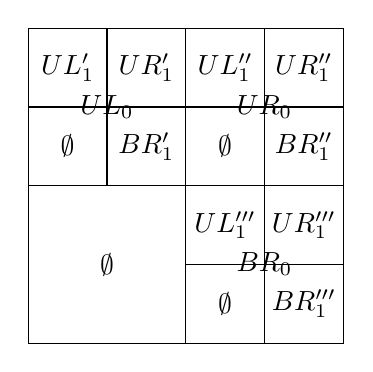
\begin{tikzpicture}[scale=0.5]
        \draw (0,0) rectangle (8,8);
    
        \draw (0,4) -- (8,4);
        \draw (4,0) -- (4,8);
        \node at (2,2) {$\emptyset$};
        
        \draw (0,6) -- (4,6);
        \draw (2,8) -- (2,4);
        \node at (1,5) {$\emptyset$};
    
        \draw (4,2) -- (8,2);
        \draw (6,4) -- (6,0);
        \node at (5,1) {$\emptyset$};

        \draw (4,6) -- (8,6);
        \draw (6,4) -- (6,8);
        \node at (5,5) {$\emptyset$};
        
        % \draw (0,7) -- (2,7);
        % \draw (1,8) -- (1,6);
        
        % \draw (2,5) -- (4,5);
        % \draw (3,6) -- (3,4);
    
        % \draw (4,3) -- (6,3);
        % \draw (5,2) -- (5,4);
        
        % \draw (6,1) -- (8,1);
        % \draw (7,0) -- (7,2);
    
        % \node at (6.5,0.5) {$\emptyset$};
        % \node at (4.5,2.5) {$\emptyset$};
        % \node at (2.5,4.5) {$\emptyset$};
        % \node at (0.5,6.5) {$\emptyset$};
    
        \node at (6,6) {$UR_0$};
        \node at (3,7) {$UR_1'$};
        \node at (7,7) {$UR_1''$};
        \node at (7,3) {$UR_1'''$};
        % \node at (1.5,7.5) {$UR_2$};
        % \node at (3.5,5.5) {$UR_2$};
        % \node at (5.5,3.5) {$UR_2$};
        % \node at (7.5,1.5) {$UR_2$};

        \node at (2,6) {$UL_0$};
        \node at (1,7) {$UL_1'$};
        \node at (5,7) {$UL_1''$};
        \node at (5,3) {$UL_1'''$};
        % \node at (0.5,7.5) {$UL_2$};
        % \node at (4.5,3.5) {$UL_2$};
        % \node at (2.5,5.5) {$UL_2$};
        % \node at (6.5,1.5) {$UL_2$};

        \node at (6,2) {$BR_0$};
        \node at (3,5) {$BR_1'$};
        \node at (7,5) {$BR_1''$};
        \node at (7,1) {$BR_1'''$};
        % \node at (7.5,0.5) {$BR_2$};
        % \node at (3.5,4.5) {$BR_2$};
        % \node at (5.5,2.5) {$BR_2$};
        % \node at (1.5,6.5) {$BR_2$};
    \end{tikzpicture}
    \caption{Two steps of recursive decomposition}
    \label{fig:qubo}
\end{figure}

The QUBO matrix is recursively divided into four parts with the following characteristics:
\begin{enumerate*}
    \item $UL$ and $BR$ are themselves QUBO matrices operating on a partition of the optimization variables,
    \item $UR$ is not guaranteed to be upper triangular and retains the information linking the two partitions of the variables,
    \item $\emptyset$ is a matrix composed entirely of zeros and can thus be ignored.
\end{enumerate*}

Figure \ref{fig:qubo} intuitively illustrates how the QUBO matrix is partitioned. Specifically, two steps are performed, reducing the single problem solved via QPU to $\frac{1}{16}$ of its original size.

The recursive subdivision continues until the matrices reach a predetermined size, which, for the data in Table \ref{tab:embedding}, could be set to 32. Focusing on the resolution of $UL_1'$, $UR_1'$ and $BR_1'$ helps understand how the proposed solution addresses the subproblems and assembles the overall solution. A similar approach applies to all other recursive steps and sections of the problem. 

Assuming that the matrices considered above are of a size that allows direct resolution on the QPU:
\begin{enumerate*}
\item $UL_1'$ and $BR_1'$ can be solved independently and their results combined to generate conflict-free initial assignments.
\item $UR_1'$ connects the two variable partitions. In practice, it is solved by incorporating the coefficients of a matrix of zeros of size $UL_0$. Although this could lead to matrices larger than the bounds tested in table \ref{tab:embedding}, the construction of this problem ensures that the resulting graph is small enough to allow for manageable computation times.
\end{enumerate*}

The two sets of solutions are combined by searching for the most compatible assignments and marking the conflicting variables. From the conflicting values, a QUBO problem is extracted, considering only the rows and columns associated with these variables, which is solved via QPU.

The proposed method of resolving conflicting assignments could, in the worst case, require reconsideration of the entire problem \(UL_0\), nullifying the decomposition process and leading to intractable cases. However, the tests have indicated that the number of conflicting variables is limited, allowing this approach to be used effectively in practice. 

From the set of possible assignments, duplicates are removed and only the $k$ most promising assignments are retained. This is to avoid an exponential increase in the number of solutions to be aggregated.

Given the non-deterministic nature of the search, it is not possible to guarantee how far the proposed solution might deviate from the optimal. Table \ref{tab:qsplit} shows the average results obtained from multiple algorithm executions on 128 variable cliques. The column ``stop dim'' indicates the size of the QUBO sub-matrix at which the direct solver is invoked via QPU. At the same time, the ``estimated range'' is the minimum and maximum energy value from 500,000 random assignments. It can be observed that, although not reaching the optimum, our proposed procedure quickly diverges from high-energy assignments, favouring lower-entropy solutions. Considering the values of ``stop dim'', it is apparent that as the size of the sub-problem solved by the QPU decreases:
\begin{enumerate*}
    \item the total calculation time required slightly increases,
    \item the approximation of the result improves.
\end{enumerate*}
The reported times do not include the computation of the minor embedding, but only the actual resolution. If the total time were considered, the proposed algorithm would be faster than direct resolution in every tested context.

\begin{table}
    \centering
    \begin{tabular}{cccccc}
        \toprule
        Stop dim & Time (s) & Proposed solution & Direct time (s) & Real sample mean & Estimated range \\
        \midrule
        2 & 75.57 & -626.71 & 51.7 & -1321.91 & -665.52, 282.35 \\
        4 & 57.19 & -674.29 & 50.92 & -1196.69 & -610.99, 292.62 \\
        8 & 50.33 & -95 & 52.31 & -958.78 & -440.96, 449.74 \\
        16 & 37.55 & -127.61 & 53.72 & -868.28 & -412.46, 447.15 \\
        32 & 32.94 & -122.6 & 51.51 & -1024.12 & -409.88, 388.24 \\
        % 64 & 48 & -118.24 & 53.87 & -854.4 & -303.07, 459.94 \\
        \bottomrule
    \end{tabular}
    \caption{Results for 128 variables cliques}
    \label{tab:qsplit}
\end{table}

\section{Conclusion}

Quantum computing for solving optimization problems brings tangible benefits over traditional methods. The trade-off between the speed of finding a solution and the quality of the results is crucial and must be evaluated on a case-by-case basis.

In many application scenarios, large computational resources are not available, such as in personal computers or embedded systems. In these situations, hybrid solvers allow for a good approximation of results while significantly reducing complexity.

The proposed strategy presents a method for handling large QUBO problems that is alternative to those found in the literature\cite{subqubo1}\cite{subqubo2}. The results of our proposed solution can be improved by implementing strategies for partitioning the QUBO matrix. One example could be considering the number of non-zero values in calculating the stop criterion. To further refine the solution produced, greater utilisation of the classical component can be considered. Currently, the algorithm focuses on maximising the use of the QPU. Although this approach is reasonable, it is not guaranteed to lead to an optimal result. For example, the assignment produced by the current algorithm could be used to initialise classical local search, such as Tabu Search\cite{tabu}, which was used by D-Wave in its early versions of hybrid solvers\cite{dwavehybrid}.
\end{spacing}

\bibliography{bibliography}

\end{document}